\documentclass{article}
\usepackage{amsmath,amssymb,graphicx,enumitem,wrapfig}

\begin{document}
\parindent=0cm
\parskip=6pt
\pagestyle{empty}

%Begin
%Language English
%Source Cariboo College High School Mathematics competition
%Title Senior Preliminary Round 1974
%Question 1
%Subject arithmetic
%Category fractions
%Type MC
%Choices 5
%Answer A
%Creator Victor Semenoff
%Rdifficulty 15
%Qtext

\scriptsize
Source: Cariboo College High School Mathematics Contest

\normalsize
%\begin{wrapfigure}[2]{r}[0pt]{0pt}
%	\includegraphics[width=30mm,viewport=]{CCJ78-04}
%\end{wrapfigure}
If $a=2.99$, then the value of $\frac{9-a^{2}}{3+a}$ is:\\
%ChoiceA
(A) .01\\
%ChoiceB
(B) .014\\
%ChoiceC
(C) .1\\
%ChoiceD
(D) 3\\
%ChoiceE
(E) 5.99\\
%Ftext

%\begin{wrapfigure}{r}[0pt]{0pt}
%	\includegraphics[width=30mm,viewport=]{CCJ78-04}
%\end{wrapfigure}

\textbf{The correct answer is (A): .01}\\[1 ex]
\begin{equation*}
\frac{9-a^{2}}{3+a}=\frac{(3-a)(3+a)}{3+a}=3-a=3-2.99=.01
\end{equation*}
%End
\\[5 ex]
%Begin
%Language English
%Source Cariboo College High School Mathematics competition
%Title Junior Preliminary Round 1973
%Question 2
%Subject geometry
%Category area
%Type MC
%Choices 5
%Answer D
%Creator Victor Semenoff
%Rdifficulty 20
%Qtext

\scriptsize
Source: Cariboo College High School Mathematics Contest

\normalsize
\begin{wrapfigure}[2]{r}[0pt]{0pt}
	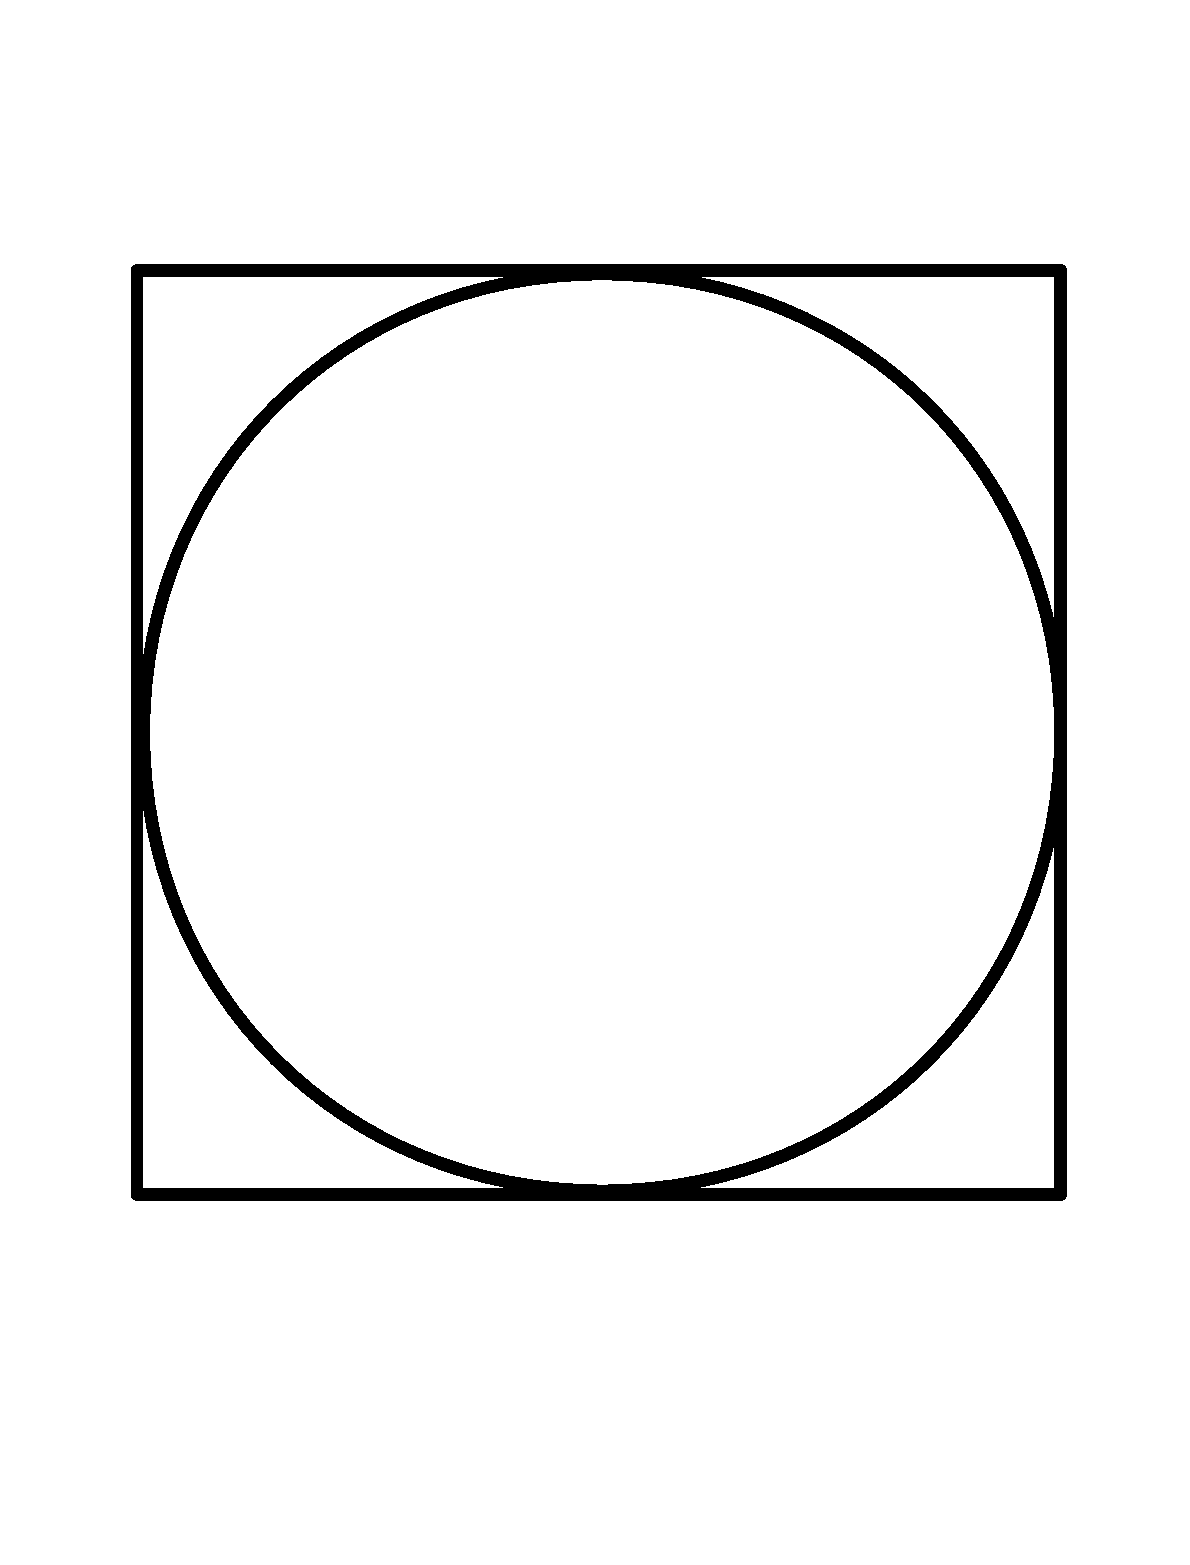
\includegraphics[width=30mm,viewport=47 157 506 618]{CCSPR74-2pic.eps}
\end{wrapfigure}
The area of the circle is $50\pi$. The side length of the square is:\\
%ChoiceA
(A) 5\\
%ChoiceB
(B) $5\sqrt{2}$\\
%ChoiceC
(C) 10\\
%ChoiceD
(D) $10\sqrt{2}$\\
%ChoiceE
(E) $10\pi$\\
%Ftext

\begin{wrapfigure}{r}[0pt]{0pt}
	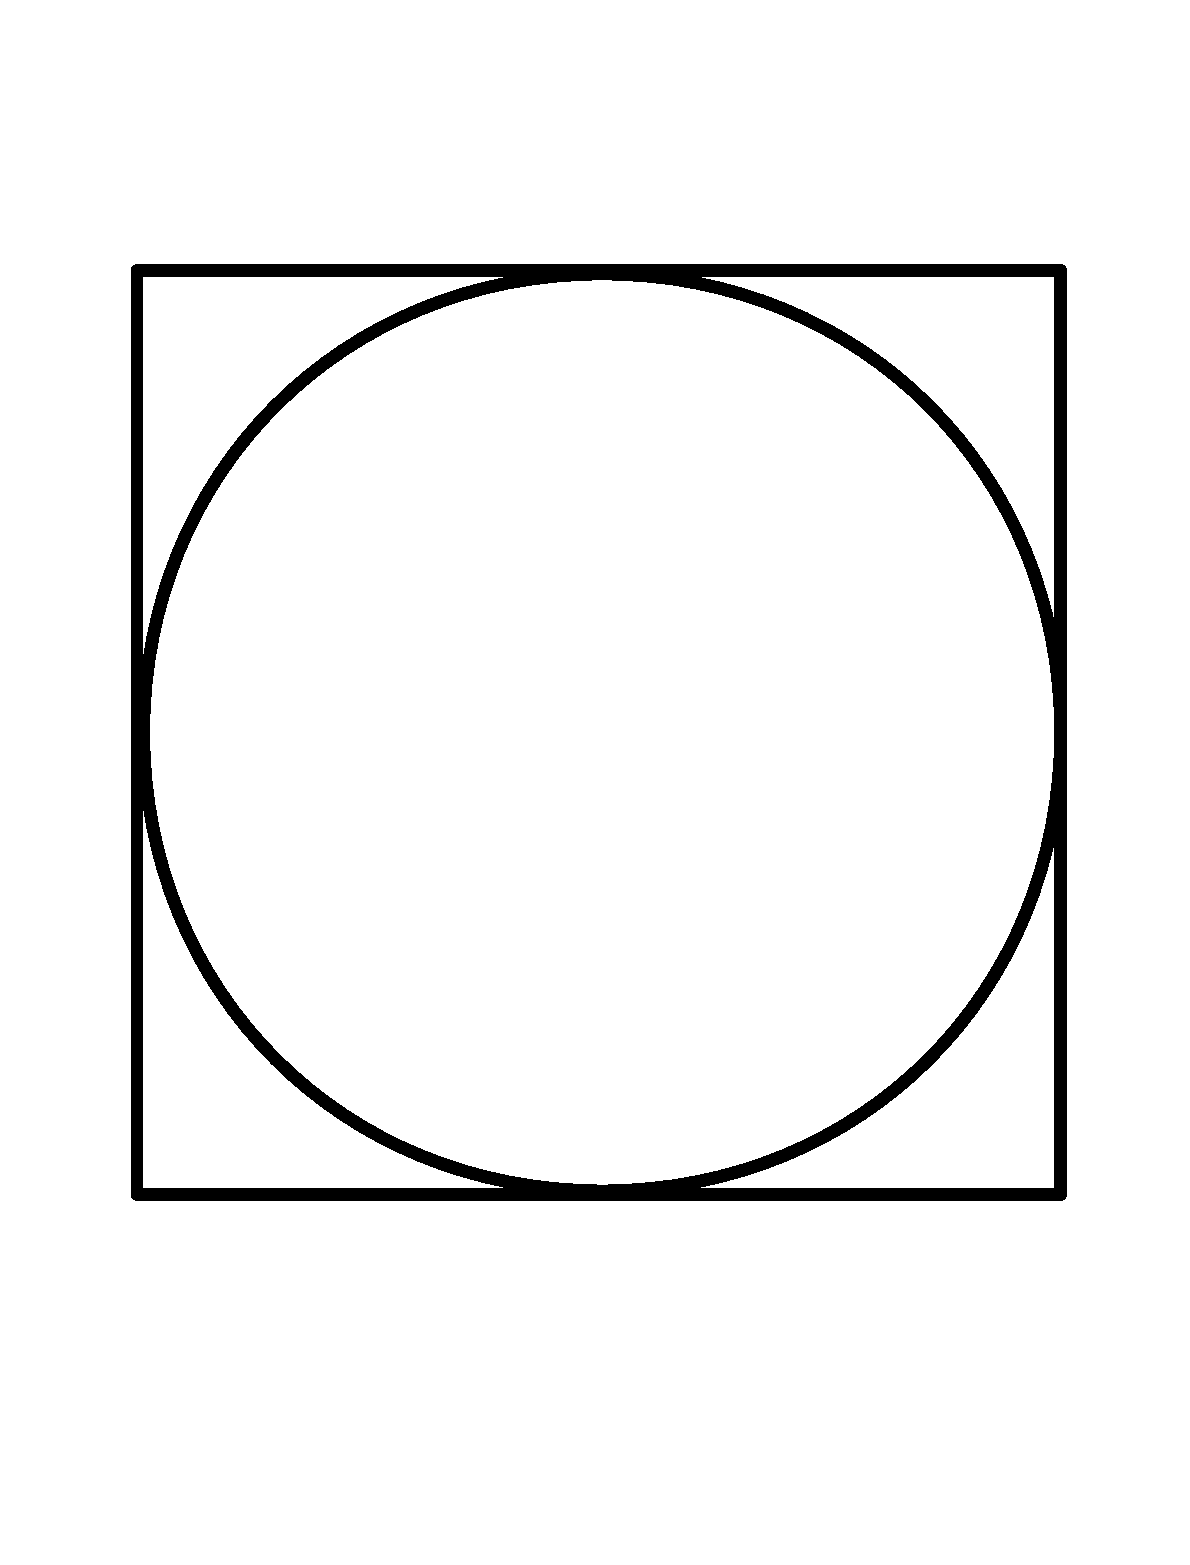
\includegraphics[width=30mm,viewport=47 157 506 618]{CCSPR74-2pic.eps}
\end{wrapfigure}

\textbf{The correct answer is (D): $10\sqrt{2}$}\\
Let $r$ be the radius of the circle. Since the area of the circle is $50\pi$, we have $\pi r^{2}=50\pi$, from which we find that $r=5\sqrt{2}$. The length of each side of the square is thus $2r$ or $10\sqrt{2}$.
%End
\\[5 ex]
%Begin
%Language English
%Source Cariboo College High School Mathematics competition
%Title Junior Preliminary Round 1973
%Question 3
%Subject geometry
%Category 3D
%Type MC
%Choices 5
%Answer D
%Creator Victor Semenoff
%Rdifficulty 22
%Qtext

\scriptsize
Source: Cariboo College High School Mathematics Contest

\normalsize
%\begin{wrapfigure}[2]{r}[0pt]{0pt}
%	\includegraphics[width=30mm]{CCJ78-04}
%\end{wrapfigure}
Six cubes are piled one on top of the other. The volume of the top cube is 16, and the volume of each of the other cubes is twice that of the one above. How long is the edge of the bottom cube?\\
%ChoiceA
(A) 64\\
%ChoiceB
(B) 32\\
%ChoiceC
(C) 16\\
%ChoiceD
(D) 8\\
%ChoiceE
(E) None of these.\\
%Ftext

%\begin{wrapfigure}{r}[0pt]{0pt}
%	\includegraphics[width=30mm]{CCJ78-04}
%\end{wrapfigure}

\textbf{The correct answer is (D): 8}\\
Let $V_n$ be the volume of the $n^{th}$ cube (counting from the top). From the question we see that $V_{1}=16$, $V_{2}=2\times V_{1}$,..., $V_{n}=2^{n-1}V_{1}$. Thus the volume of the $6^{th}$ cube is
\begin{equation*}
V_{6}=2^{5}V_{1}=32\times16=2^9
\end{equation*}
If $l$ is the length of the side of this cube, the last equation gives $l^{3}=2^9$, from which we find that $l=8$.
%End
\\[5 ex]
%Begin
%Language English
%Source Cariboo College High School Mathematics competition
%Title Junior Preliminary Round 1973
%Question 4
%Subject functions
%Category rational
%Type MC
%Choices 5
%Answer E
%Creator Victor Semenoff
%Rdifficulty 20
%Qtext
\scriptsize
Source: Cariboo College High School Mathematics Contest

\normalsize
%\begin{wrapfigure}[2]{r}[0pt]{0pt}
%	\includegraphics[width=30mm]{CCJ78-04}
%\end{wrapfigure}
If $\frac{x-y}{x+y}=\frac{12}{13}$, then $\frac{x^2}{y^2}$:\\
%ChoiceA
(A) $\frac{12}{13}$\\[1 ex]
%ChoiceB
(B) $\frac{25}{6}$\\[1 ex]
%ChoiceC
(C) $\frac{144}{169}$\\[1 ex]
%ChoiceD
(D) $\frac{25}{1}$\\[1 ex]
%ChoiceE
(E) $\frac{625}{1}$\\
%Ftext

%\begin{wrapfigure}{r}[0pt]{0pt}
%	\includegraphics[width=30mm]{CCJ78-04}
%\end{wrapfigure}

\textbf{The correct answer is (E): $\frac{625}{1}$}\\
\begin{align*}
\frac{x-y}{x+y}&=\frac{12}{13}\\
13x-13y&=12x+12y\\
x&=25y\\
x^{2}&=(25)^{2}y^2\\
\frac{x^2}{y^2}=\frac{625}{1}
\end{align*}
%End
\\[5 ex]
%Begin
%Language English
%Source Cariboo College High School Mathematics competition
%Title Junior Preliminary Round 1973
%Question 5
%Subject algebra
%Category modelling
%Type MC
%Choices 5
%Answer D
%Creator Victor Semenoff
%Rdifficulty 22
%Qtext

\scriptsize
Source: Cariboo College High School Mathematics Contest

\normalsize
%\begin{wrapfigure}[2]{r}[0pt]{0pt}
%	\includegraphics[width=30mm]{CCJ78-04}
%\end{wrapfigure}
A mixture is four parts wine to eleven parts water. If there are 150 gallons of the mixture, how many gallons of wine must be added to make the mixture two parts wine to three parts water?\\
%ChoiceA
(A) 45\\
%ChoiceB
(B) 3$\frac{1}{3}$\\
%ChoiceC
(C) 20\\
%ChoiceD
(D) 33$\frac{1}{3}$\\
%ChoiceE
(E) 53$\frac{1}{3}$\\
%Ftext

%\begin{wrapfigure}{r}[0pt]{0pt}
%	\includegraphics[width=30mm]{CCJ78-04}
%\end{wrapfigure}

\textbf{The correct answer is (D): 33$\frac{1}{3}$}\\
Let $x$ be the number of gallons of wine that must be added. To begin with, $\frac{4}{15}$ of the mixture is wine, and $\frac{11}{15}$ of the mixture is water. Since there are a total of 150 gallons, this means that $\frac{4}{15}\times150=40$ gallons are wine and $\frac{11}{15}\times150=110$ are water. When the wine is added there will be $40+x$ gallons of wine, and 110 gallons of water. Since the mixture is to be 2 parts wine to 3 parts water, we need $x$ such that $40+x:110=2:3$. Thus
\begin{align*}
\frac{40+x}{110}&=\frac{2}{3}\\
120+3x&=220\\
3x&=100\\
x&=33\frac{1}{3}.
\end{align*}
%End
\\[5 ex]
%Begin
%Language English
%Source Cariboo College High School Mathematics competition
%Title Junior Preliminary Round 1973
%Question 6
%Subject functions
%Category concepts
%Type MC
%Choices 5
%Answer A
%Creator Victor Semenoff
%Rdifficulty 19
%Qtext

\scriptsize
Source: Cariboo College High School Mathematics Contest

\normalsize
%\begin{wrapfigure}[2]{r}[0pt]{0pt}
%	\includegraphics[width=30mm,viewport=]{CCJ78-04}
%\end{wrapfigure}
Let $R=\frac{6x-3}{3x}$ where $x$ is positive. Then:\\
%ChoiceA
(A) $R$ increases as $x$ increases, but $R$ never exceeds 2\\
%ChoiceB
(B) $R$ decreases as $x$ increases, but $R$ is never less than 0\\
%ChoiceC
(C) $R$ decreases as $x$ increases, but $R$ is never less than 1\\
%ChoiceD
(D) $R$ increases as $x$ decreases, but exceeds 2\\
%ChoiceE
(E) $R$ neither increases nor decreases, as $x$ increases\\
%Ftext

%\begin{wrapfigure}{r}[0pt]{0pt}
%	\includegraphics[width=30mm,viewport=]{CCJ78-04}
%\end{wrapfigure}
\textbf{The correct answer is (A): $R$ increases as $x$ increases, but $R$ never exceeds 2}\\
\begin{equation*}
R=\frac{6x-3}{3x}=\frac{2x-1}{x}=2-\frac{1}{x}
\end{equation*}
From this equation we see that as $x$ increases, the second term on the right decreases, so $R$ increases. This same term can never decrease to 0, however; therefore, $R$ can never exceed 2.
%End
\\[5 ex]
%Begin
%Language English
%Source Cariboo College High School Mathematics competition
%Title Junior Preliminary Round 1973
%Question 7
%Subject geometry
%Category triangles
%Type MC
%Choices 5
%Answer B
%Creator Victor Semenoff
%Rdifficulty 20
%Qtext

\scriptsize
Source: Cariboo College High School Mathematics Contest

\normalsize
\begin{wrapfigure}[2]{r}[0pt]{0pt}
	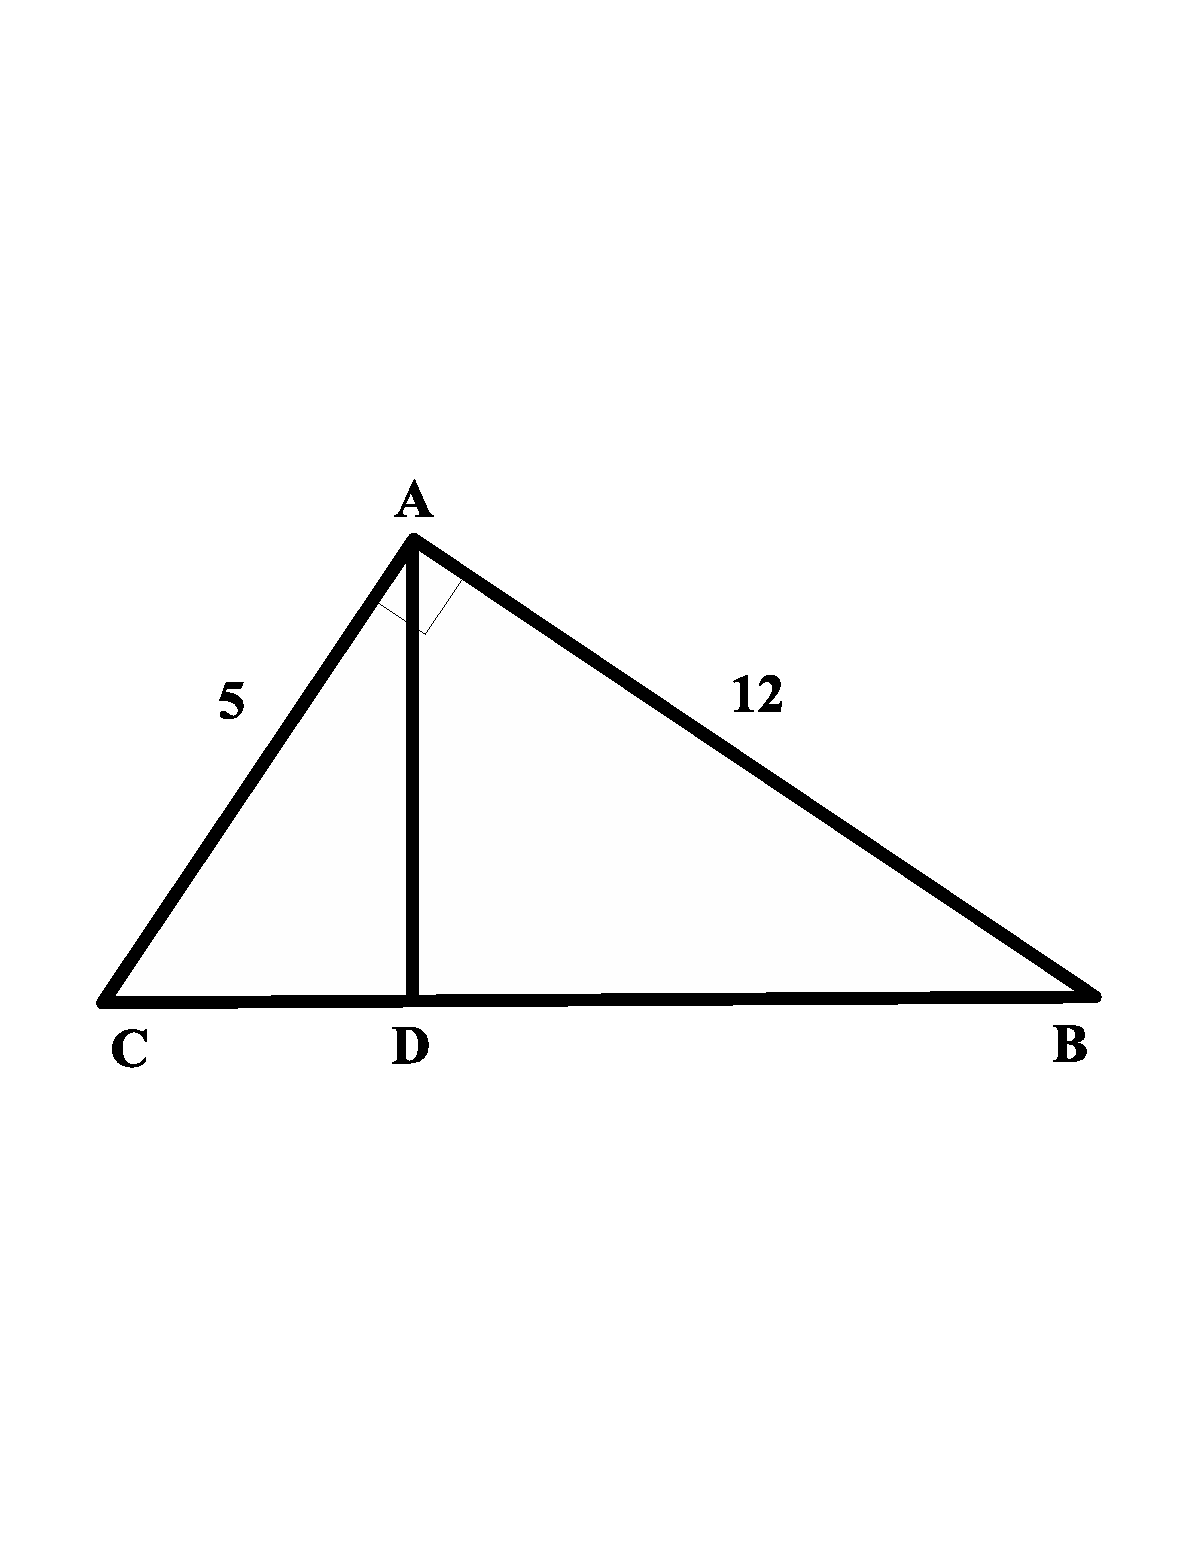
\includegraphics[width=30mm,viewport=32 226 524 516]{CCSPR74-7pic.eps}
\end{wrapfigure}
The three triangles shown in the diagram are right triangles. If AB=12 and AC=5, then the area of the smallest triangle is:\\
%ChoiceA
(A) 6\\
%ChoiceB
(B) $\frac{750}{169}$\\
%ChoiceC
(C) 10\\
%ChoiceD
(D) 12\\
%ChoiceE
(E) $\frac{150}{13}$\\
%Ftext

\begin{wrapfigure}{r}[0pt]{0pt}
	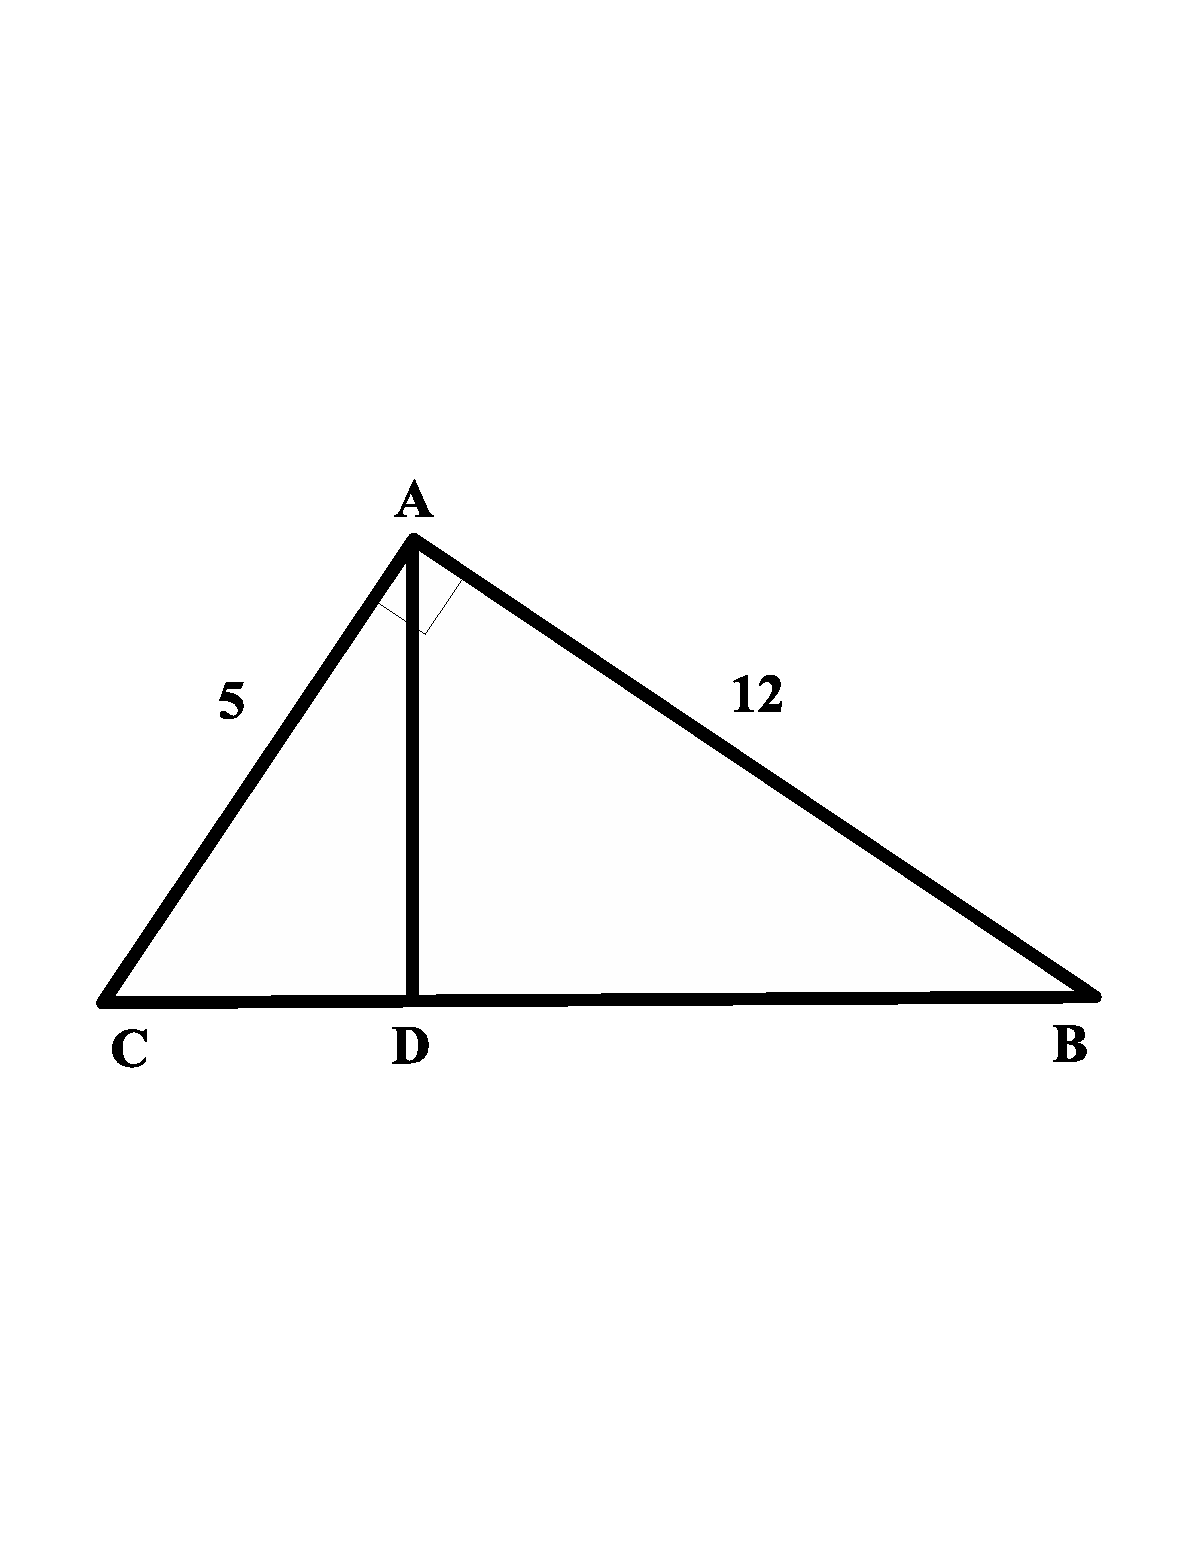
\includegraphics[width=30mm,viewport=32 226 524 516]{CCSPR74-7pic.eps}
\end{wrapfigure}

\textbf{The correct answer is (B): $\frac{750}{169}$}\\[1ex]
The hypotenuse of $\triangle$ABC is 13, and its area is $\frac{1}{2}\times5\times12=30$. Let $\alpha=\angle$ABC, and let $\beta$ be its compliment. Then $\angle$BAD$=\beta$, $\angle$CAD$=\alpha$, and $\angle$ACD$=\beta$. Since triangles ACD and ABC have two common angles, they are similar. It then follows that, since the hypotenuse of $\triangle$ACD is $\frac{5}{13}$ the length of the hypotenuse of $\triangle$ABC, the base and the height of $\triangle$ACD will be $\frac{5}{13}$ the base and the height (respectively) of $\triangle$ABC. Similarly, the area of $\triangle$ACD will be $(\frac{5}{13})^2)$ of the area of $\triangle$ABC. Thus the area of $\triangle$ACD is
\begin{equation*}
(\frac{5}{13})^{2}\times30=\frac{25\times30}{169}=\frac{750}{169}.
\end{equation*}
%End
\\[5 ex]
%Begin
%Language English
%Source Cariboo College High School Mathematics competition
%Title Junior Preliminary Round 1973
%Question 8
%Subject geometry
%Category 3D
%Type MC
%Choices 5
%Answer B
%Creator Victor Semenoff
%Rdifficulty 20
%Qtext

\scriptsize
Source: Cariboo College High School Mathematics Contest

\normalsize
%\begin{wrapfigure}[2]{r}[0pt]{0pt}
%	\includegraphics[width=30mm,viewport=]{CCJ78-04}
%\end{wrapfigure}
What fraction of a spherical orange is inedible if the outer radius of the orange is 2 inches and the skin is $\frac{1}{2}$ inches thick? (The volume of a sphere is $\frac{4}{3}\pi r^3$ and its surface area is $4\pi r^2$.)\\
%ChoiceA
(A) $\frac{3}{5}$\\[1 ex]
%ChoiceB
(B) $\frac{37}{64}$\\[1 ex]
%ChoiceC
(C) $\frac{98}{125}$\\[1 ex]
%ChoiceD
(D) $\frac{63}{64}$\\[1 ex]
%ChoiceE
(E) $\frac{27}{64}$\\
%Ftext

%\begin{wrapfigure}{r}[0pt]{0pt}
%	\includegraphics[width=30mm,viewport=]{CCJ78-04}
%\end{wrapfigure}

\textbf{The correct answer is (B): $\frac{37}{64}$}\\[1 ex]
The total volume of the orange is
\begin{equation*}
\frac{4}{3}\pi 2^3.
\end{equation*}
The edible portion of the orange is a sphere of radius $(2-\frac{1}{2})=\frac{3}{2}$, with a volume of
\begin{equation*}
\frac{4}{3}\pi(\frac{3}{2})^3.
\end{equation*}
Therefore, the volume of the inedible portion is
\begin{equation*}
\frac{4}{3}\pi 2^3-\frac{4}{3}\pi(\frac{3}{2})^3=\frac{4}{3}\pi( 2^3-(\frac{3}{2})^3).
\end{equation*}
The fraction of the orange that is inedible will equal the volume of the inedible region divided by the total volume of the orange, or
\begin{equation*}\frac{\frac{4}{3}\pi( 2^3-(\frac{3}{2})^3)}{\frac{4}{3}\pi 2^3}=\frac{( 2^3-(\frac{3}{2})^3)}{2^3}=1-\frac{27}{64}=\frac{37}{64}.
\end{equation*}
%End
\\[5 ex]
%Begin
%Language English
%Source Cariboo College High School Mathematics competition
%Title Junior Preliminary Round 1973
%Question 9
%Subject algebra
%Category modelling
%Type MC
%Choices 5
%Answer A
%Creator Victor Semenoff
%Rdifficulty 24
%Qtext

\scriptsize
Source: Cariboo College High School Mathematics Contest

\normalsize
%\begin{wrapfigure}[2]{r}[0pt]{0pt}
%	\includegraphics[width=30mm,viewport=]{CCJ78-04}
%\end{wrapfigure}
A log $12\frac{1}{2}$ft long and 30 inches in diameter lies at the top of a slope. As a girl climbs onto one end of the log and walks towards the other end, the log begins to roll down the slope. If the girl is always at the top of the log, and if the log rolls 12 yards before she jumps off the end, how many yards has she traveled\\
%ChoiceA
(A) 12$\frac{1}{2}$\\
%ChoiceB
(B) 25\\
%ChoiceC
(C) $\frac{72}{\pi}$\\
%ChoiceD
(D) $\sqrt{400\pi^{2}+49}$\\
%ChoiceE
(E) None of these.\\
%Ftext

%\begin{wrapfigure}{r}[0pt]{0pt}
%	\includegraphics[width=30mm,viewport=]{CCJ78-04}
%\end{wrapfigure}

\textbf{The correct answer is (A): 12$\frac{1}{2}$}\\[1 ex]
Let $A$ be the point where the girl got on the log, $B$ the point where she jumped off the log, and $C$ the point where the other end of the log was when she jumped off. $\triangle ABC$ is then a right triangle. $AC$ will be the distance the log moved forward, $CB$ will be the length of the log, and $AB$ will be the distance the girl traveled. By the Pythagoras theorem
\begin{align*}
(AB)^{2}&=(AC)^{2}+(CB)^{2}=(12\textrm{yd})^{2}+(12\frac{1}{2}\textrm{ft})^{2}=(12\textrm{yd})^{2}+(3\frac{1}{2}\textrm{yd})^{2}\\
&=(144+\frac{49}{4})\textrm{yd}^{2}\\
AB&=12.5\textrm{yd}.
\end{align*}
%End
\\[5 ex]
%Begin
%Language English
%Source Cariboo College High School Mathematics competition
%Title Junior Preliminary Round 1973
%Question 10
%Subject geometry
%Category length
%Type MC
%Choices 5
%Answer B
%Creator Victor Semenoff
%Rdifficulty 25
%Qtext

\scriptsize
Source: Cariboo College High School Mathematics Contest

\normalsize
\begin{wrapfigure}[2]{r}[0pt]{0pt}
	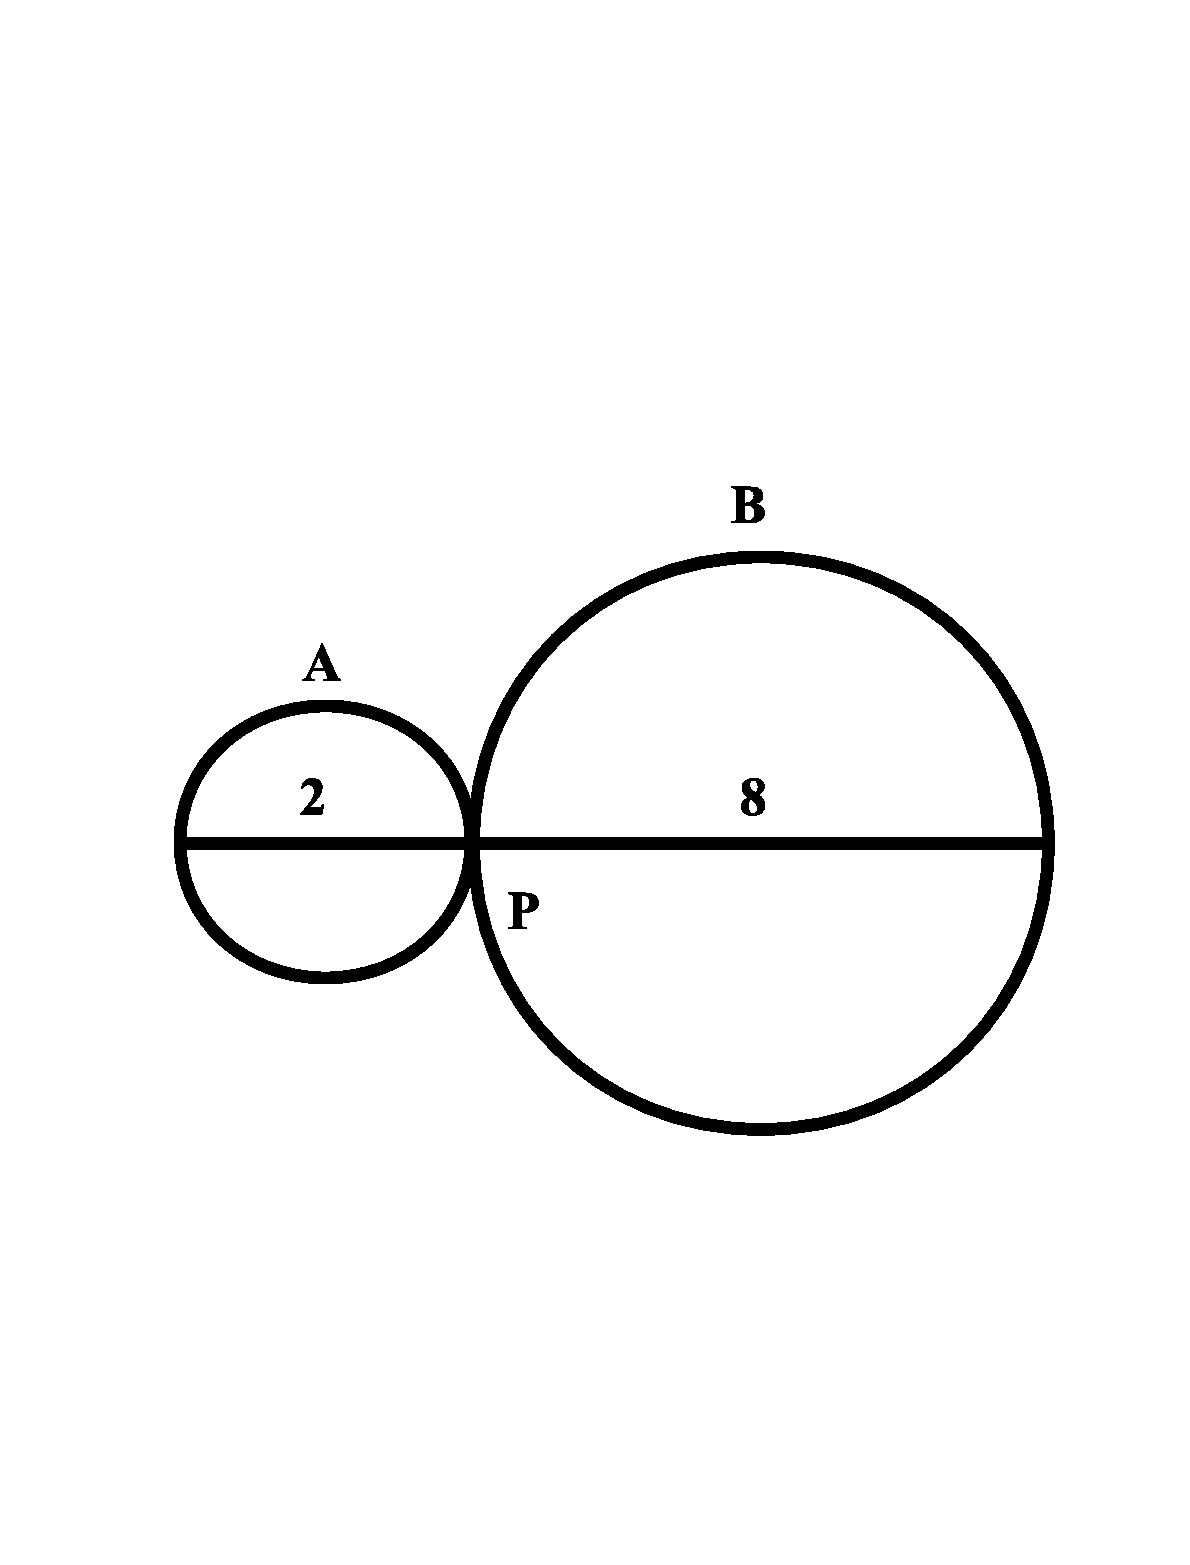
\includegraphics[width=30mm,viewport=74 194 500 512]{CCSPR74-10pic.eps}
\end{wrapfigure}
The diameters of circles $A$ and $B$ are shown. If circle $B$ is fixed, and circle $A$ rolls tangentially (without slipping), once around $B$, how many revolutions will $A$ have made?\\
%ChoiceA
(A) 9\\
%ChoiceB
(B) 6\\
%ChoiceC
(C) 3\\
%ChoiceD
(D) 5\\
%ChoiceE
(E) 8\\
%Ftext

\begin{wrapfigure}{r}[0pt]{0pt}
	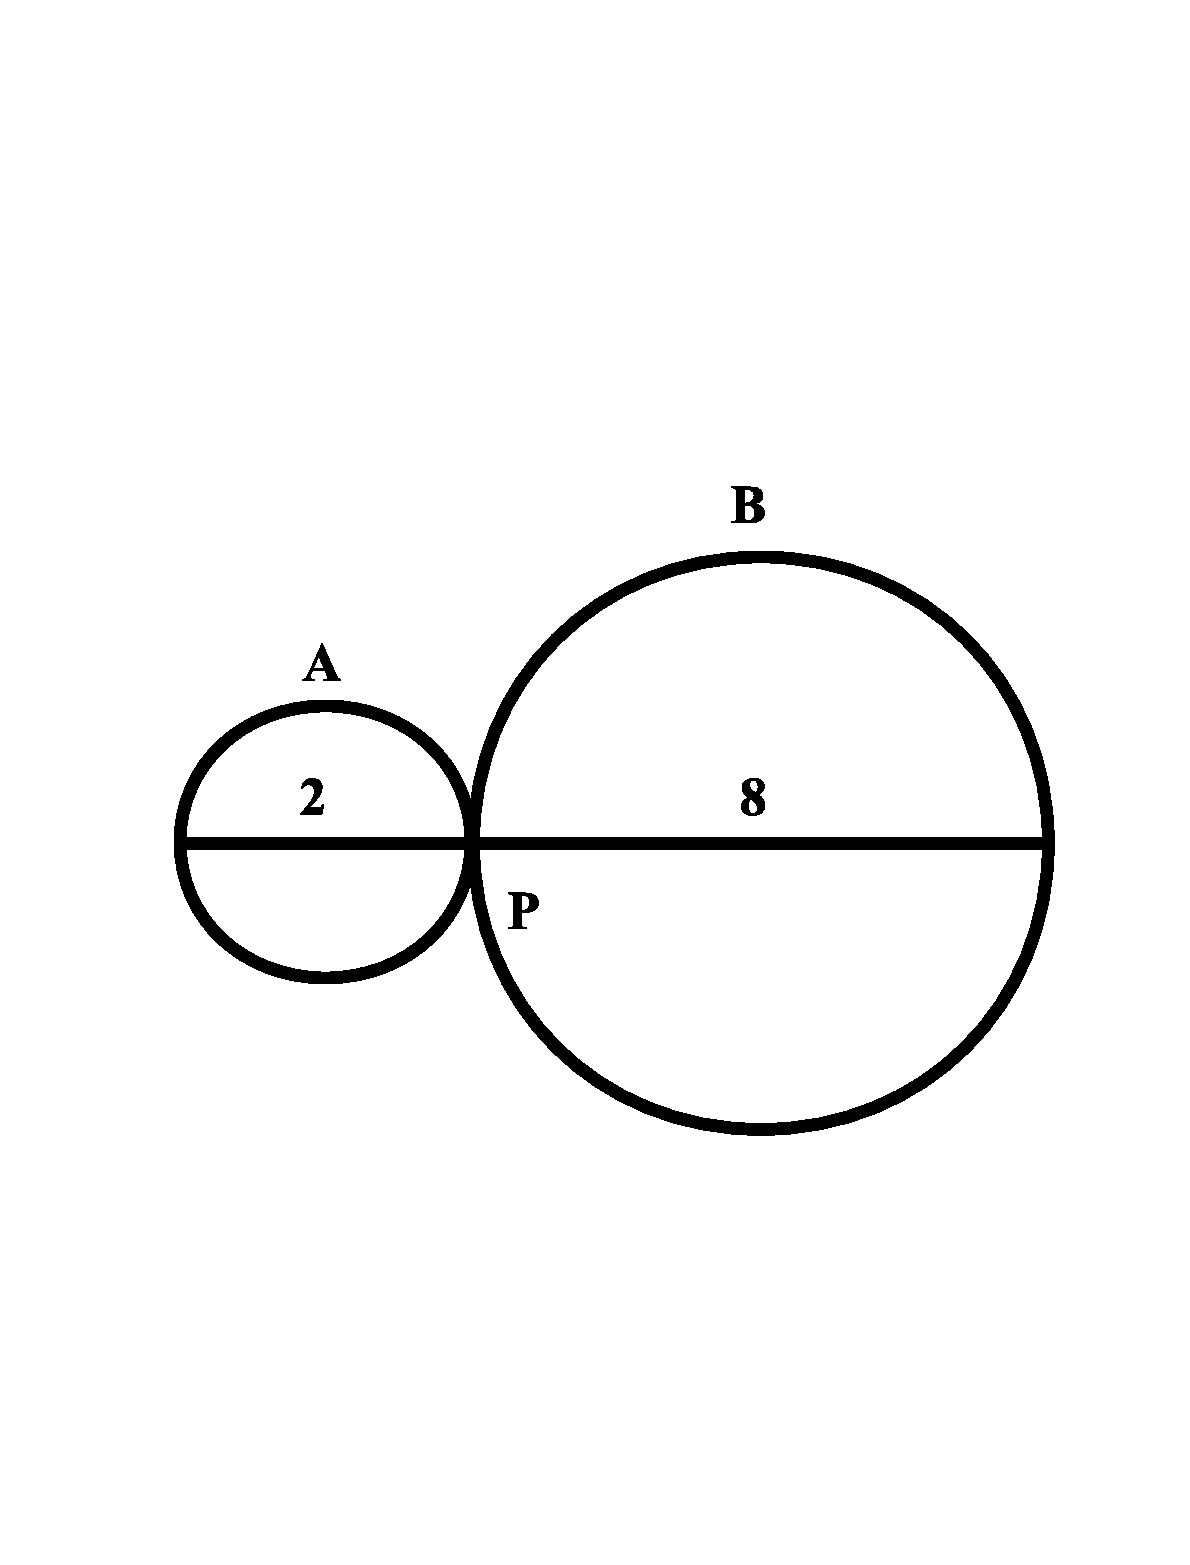
\includegraphics[width=30mm,viewport=74 194 500 512]{CCSPR74-10pic.eps}
\end{wrapfigure}

\textbf{The correct answer is (B): 6}\\[1 ex]
The small circle $A$ has circumference $2\pi$ and the large circle $B$ has circumference $8\pi$. If $A$ rolls around $B$ without slipping, then the point $P$ on $A$ travels the full circumference of $B$. Thus $P$ travels $8\pi$, which is 4 circumferences of the circle $A$.

In addition, if there was slipping and no spinning of $A$ (point $P$ always in contact with $B$). Then the point $P$ has made 1 full rotation around $A$ as it traversed $B$.

Putting them together we get there are $4+1=5$ rotations.
%End
\\[5 ex]
%Begin
%Language English
%Source Cariboo College High School Mathematics competition
%Title Junior Preliminary Round 1973
%Question 11
%Subject geometry
%Category 3D
%Type MC
%Choices 5
%Answer D
%Creator Victor Semenoff
%Rdifficulty 22
%Qtext

\scriptsize
Source: Cariboo College High School Mathematics Contest

\normalsize
%\begin{wrapfigure}[2]{r}[0pt]{0pt}
%	\includegraphics[width=30mm,viewport=]{CCJ78-04}
%\end{wrapfigure}
A lead sphere of radius 9mm and another sphere of radius 10mm are melted down and the lead is used to make two new spheres. The radius of one of these new spheres is 1mm; the radius of the other (in mm) is then:\\
%ChoiceA
(A) 18$\frac{1}{2}$\\
%ChoiceB
(B) 14\\
%ChoiceC
(C) 14.5\\
%ChoiceD
(D) 12\\
%ChoiceE
(E) 9.5\\
%Ftext

%\begin{wrapfigure}{r}[0pt]{0pt}
%	\includegraphics[width=30mm,viewport=]{CCJ78-04}
%\end{wrapfigure}

\textbf{The correct answer is (D): 12}\\[1 ex]
Let $r$ be the radius of the new sphere. Its volume is $\frac{4}{3}\pi r^3$, while volumes of the 9mm, 10mm, and 1mm spheres are $\frac{4}{3}\pi 9^3$, $\frac{4}{3}\pi 10^3$, $\frac{4}{3}\pi 1^3$
respectively. Thus the total volume of the two original spheres is
\begin{equation*}
\frac{4}{3}\pi 9^3+\frac{4}{3}\pi 10^3
\end{equation*}
while the total volume of the new spheres is
\begin{equation*}
\frac{4}{3}\pi 1^3+\frac{4}{3}\pi r^3.
\end{equation*}
Assuming no metal is lost, the original total volume is equal to the new total volume, thus
\begin{align*}
\frac{4}{3}\pi 9^3+\frac{4}{3}\pi 10^3&=\frac{4}{3}\pi 1^3+\frac{4}{3}\pi r^3\\
r^{3}&=9^{3}+10^{3}-1^{3}=1728\\
r&=12.
\end{align*}
%End
\\[5 ex]
%Begin
%Language English
%Source Cariboo College High School Mathematics competition
%Title Junior Preliminary Round 1973
%Question 12
%Subject functions
%Category concepts
%Type MC
%Choices 5
%Answer A
%Creator Victor Semenoff
%Rdifficulty 23
%Qtext

\scriptsize
Source: Cariboo College High School Mathematics Contest

\normalsize
%\begin{wrapfigure}[2]{r}[0pt]{0pt}
%	\includegraphics[width=30mm,viewport=]{CCJ78-04}
%\end{wrapfigure}
If $ax^{3}+bx-2=0$ for $x=-1$, what is the value of $ax^{3}+bx-2$ for $x=1$?\\
%ChoiceA
(A) -4\\
%ChoiceB
(B) -2\\
%ChoiceC
(C) 0\\
%ChoiceD
(D) 2\\
%ChoiceE
(E) 4\\
%Ftext

%\begin{wrapfigure}{r}[0pt]{0pt}
%	\includegraphics[width=30mm,viewport=]{CCJ78-04}
%\end{wrapfigure}

\textbf{The correct answer is (A): -4}\\[1 ex]
Since $ax^{3}+bx-2=0$ when $x=-1$, we have
\begin{align*}
a(-1)^{3}+b(-1)-2&=0\\
-a-b-2&=0\\
a+b&=-2.
\end{align*}
Therefore, when $x=1$, $ax^{3}+bx-2=0$ becomes
\begin{equation*}
a(1)^{3}+b(1)-2=a+b-2=-2-2=-4.
\end{equation*}
%End
\\[5 ex]
%Begin
%Language English
%Source Cariboo College High School Mathematics competition
%Title Junior Preliminary Round 1973
%Question 13
%Subject functions
%Category concepts
%Type MC
%Choices 5
%Answer E
%Creator Victor Semenoff
%Rdifficulty 24
%Qtext

\scriptsize
Source: Cariboo College High School Mathematics Contest

\normalsize
%\begin{wrapfigure}[2]{r}[0pt]{0pt}
%	\includegraphics[width=30mm,viewport=]{CCJ78-04}
%\end{wrapfigure}
Which of the following is not a factor of $4a^{2}c^{2}-(a^{2}+c^{2}-b^{2}))^2$?\\
%ChoiceA
(A) $a+b+c$\\
%ChoiceB
(B) $a-b-c$\\
%ChoiceC
(C) $a+b-c$\\
%ChoiceD
(D) $a-b+c$\\
%ChoiceE
(E) They are all factors.\\
%Ftext

%\begin{wrapfigure}{r}[0pt]{0pt}
%	\includegraphics[width=30mm,viewport=]{CCJ78-04}
%\end{wrapfigure}

\textbf{The correct answer is (E): They are all factors.}\\[1 ex]
Using the fact that $x^2-y^2=(x+y)(x-y)$, we find
\begin{align*}
4a^{2}c^{2}-(a^2+c^2-b^2)^2&=(2ac +a^2+c^2-b^2)(2ac-a^2-c^2+b^2)\\
&=-(2ac +a^2+c^2)(-2ac+a^2+c^2-b^2)\\
&=-((a+c)^2-b^2)((a-c)^2-b^2)\\
&=(a+c-b)(a+c+b)(a-b-c)(a+b-c).
\end{align*}
Therefore, all the answers given are factors of $4a^{2}c^{2}-(a^2+c^2-b^2)^2$.
%End
\\[5 ex]
%Begin
%Language English
%Source Cariboo College High School Mathematics competition
%Title Junior Preliminary Round 1973
%Question 14
%Subject arithmetic
%Category fractions
%Type MC
%Choices 5
%Answer E
%Creator Victor Semenoff
%Rdifficulty 22
%Qtext

\scriptsize
Source: Cariboo College High School Mathematics Contest

\normalsize
%\begin{wrapfigure}[2]{r}[0pt]{0pt}
%	\includegraphics[width=30mm,viewport=]{CCJ78-04}
%\end{wrapfigure}
For what real values of $x$ is $y=\frac{\sqrt{4-x^2}}{x^2+3x}$ a real number?\\
%ChoiceA
(A) $-2\leq x\leq2$\\
%ChoiceB
(B) $x\neq3$\\
%ChoiceC
(C) $-x<2$,$x>2$\\
%ChoiceD
(D) $x\neq0$\\
%ChoiceE
(E) $-2\leq x\leq 2$,$x\neq0$\\
%Ftext

%\begin{wrapfigure}{r}[0pt]{0pt}
%	\includegraphics[width=30mm,viewport=]{CCJ78-04}
%\end{wrapfigure}

\textbf{The correct answer is (E): $-2\leq x\leq 2$,$x\neq0$}\\[1 ex]
y will be undefined when the denominator, $x^2+3x$ is 0. This occurs when
\begin{align*}
x^2+3x&=0\\
x(x+3)&=0,
\end{align*}
or at $x=0$ and $x=-3$. The numerator, $\sqrt{4-x^2}$, is real when $4-x^2\geq0$, or $-2\leq x\leq 2$. Therefore $y$ is real when $-2\leq x\leq 2$ and $x\neq0$.
%End
\\[5 ex]
%Begin
%Language English
%Source Cariboo College High School Mathematics competition
%Title Junior Preliminary Round 1973
%Question 15
%Subject functions
%Category concepts
%Type MC
%Choices 5
%Answer A
%Creator Victor Semenoff
%Rdifficulty 24
%Qtext

\scriptsize
Source: Cariboo College High School Mathematics Contest

\normalsize
%\begin{wrapfigure}[2]{r}[0pt]{0pt}
%	\includegraphics[width=30mm,viewport=]{CCJ78-04}
%\end{wrapfigure}
If $3x^2-mx^2+4x+5$ is divisible by $x+1$, then $m$ equals:\\
%ChoiceA
(A) -2\\
%ChoiceB
(B) 3\\
%ChoiceC
(C) -4\\
%ChoiceD
(D) 0\\
%ChoiceE
(E) None of these.\\
%Ftext

%\begin{wrapfigure}{r}[0pt]{0pt}
%	\includegraphics[width=30mm,viewport=]{CCJ78-04}
%\end{wrapfigure}

\textbf{The correct answer is (A): -2}\\[1 ex]
Let $f(x)=3x^2-mx^2+4x+5$. Then according to the factor theorem, $x+1$ will be a factor of $f(x)$ when $f(-1)=0$. Thus we need $m$ such that 
\begin{equation*}
f(-1)=-3-m-4+5=0.
\end{equation*}
Thus $m=-2$.
%End
\\[5 ex]
%Begin
%Language English
%Source Cariboo College High School Mathematics competition
%Title Junior Preliminary Round 1973
%Question 16
%Subject geometry
%Category pythagorus
%Type MC
%Choices 5
%Answer B
%Creator Victor Semenoff
%Rdifficulty 21
%Qtext

\scriptsize
Source: Cariboo College High School Mathematics Contest

\normalsize
%\begin{wrapfigure}[2]{r}[0pt]{0pt}
%	\includegraphics[width=30mm,viewport=]{CCJ78-04}
%\end{wrapfigure}
Antonio travels due north at 5 mi/h on a flat plain. Betty travels due east on the same plain at 10 mi/h. In how many hours will the distance between them be 20 miles, if they start at the same time from the same point?\\
%ChoiceA
(A) $\frac{4}{3}$\\
%ChoiceB
(B) $\frac{4\sqrt{5}}{5}$\\
%ChoiceC
(C) $\frac{4}{3}\sqrt{15}$\\
%ChoiceD
(D) $4(\sqrt{10}-\sqrt{5})$\\
%ChoiceE
(E) $4\sqrt{5}$\\
%Ftext

%\begin{wrapfigure}{r}[0pt]{0pt}
%	\includegraphics[width=30mm,viewport=]{CCJ78-04}
%\end{wrapfigure}

\textbf{The correct answer is (B): $\frac{4\sqrt{5}}{5}$}\\[1 ex]
Let $t$ be the number of hours we seek. In this time Antonio will be $5t$ miles north of the starting point and Betty will be $10t$ miles east.  Their positions and the origin form a right triangle with the hypotenuse being the distance between them. Thus we are looking for $t$ such that 
\begin{align*}
20&=\sqrt{(5t)^2+(10t)^2}\\
20^2&=125t^2\\
t^2&=\frac{20^2}{125}\\
t&=\frac{20}{5\sqrt{5}}=\frac{4\sqrt{5}}{5}.
\end{align*}
%End
\\[5 ex]
%Begin
%Language English
%Source Cariboo College High School Mathematics competition
%Title Junior Preliminary Round 1973
%Question 17
%Subject functions
%Category concepts
%Type MC
%Choices 5
%Answer C
%Creator Victor Semenoff
%Rdifficulty 24
%Qtext

\scriptsize
Source: Cariboo College High School Mathematics Contest

\normalsize
%\begin{wrapfigure}[2]{r}[0pt]{0pt}
%	\includegraphics[width=30mm,viewport=]{CCJ78-04}
%\end{wrapfigure}
If $f(-x)=-f(x)$ for all $x$, and $f(3)=5$, then $\frac{f(3)-f(-3)}{2}+f(0)$ equals:\\
%ChoiceA
(A) -5\\
%ChoiceB
(B) 0\\
%ChoiceC
(C) 5\\
%ChoiceD
(D) 8\\
%ChoiceE
(E) Not enough information.\\
%Ftext

%\begin{wrapfigure}{r}[0pt]{0pt}
%	\includegraphics[width=30mm,viewport=]{CCJ78-04}
%\end{wrapfigure}

\textbf{The correct answer is (C): 5}\\[1 ex]
From the definition of $f(-x)$, it follows that $f(-0)=-f(0)=f(0)$, thus $f(0)=0$. Then
\begin{equation*}
\frac{f(3)-f(-3)}{2}+f(0)=\frac{f(3)-f(-3)}{2}=\frac{2f(3)}{2}=f(3)=5.
\end{equation*}
%End
\\[5 ex]
%Begin
%Language English
%Source Cariboo College High School Mathematics competition
%Title Junior Preliminary Round 1973
%Question 18
%Subject geometry
%Category length
%Type MC
%Choices 5
%Answer A
%Creator Victor Semenoff
%Rdifficulty 27
%Qtext

\scriptsize
Source: Cariboo College High School Mathematics Contest

\normalsize
\begin{wrapfigure}[2]{r}[0pt]{0pt}
	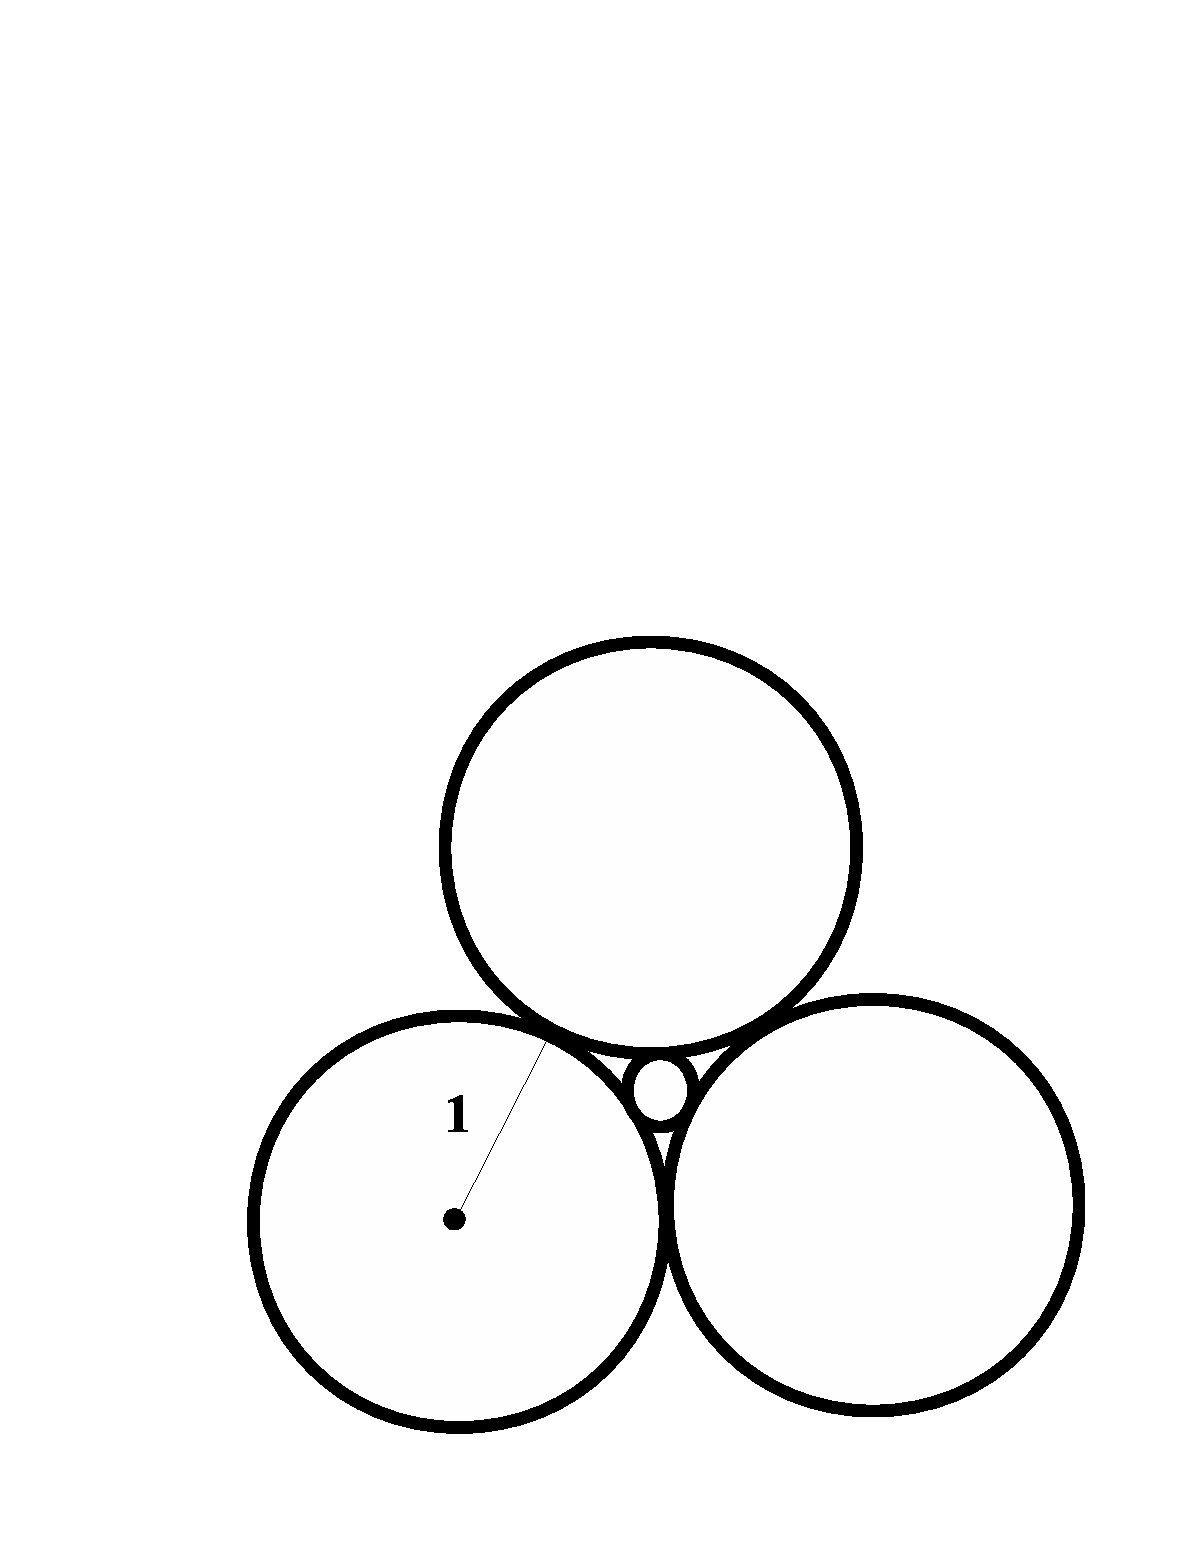
\includegraphics[width=30mm,viewport=106 49 515 440]{CCSPR74-18pic.eps}
\end{wrapfigure}
The three larger circles, all of radius 1, are tangent to each other. The radius of the smaller circle is:\\
%ChoiceA
(A) $\frac{2\sqrt{3}-3}{3}$\\[1 ex]
%ChoiceB
(B) $\frac{2\sqrt{3}+3}{3}$\\[1 ex]
%ChoiceC
(C) $\frac{2}{\sqrt{3}}$\\[1 ex]
%ChoiceD
(D) $\frac{\sqrt{5}-1}{2}$\\[1 ex]
%ChoiceE
(E) $\frac{\sqrt{5}-2}{3}$\\
%Ftext

\begin{wrapfigure}{r}[0pt]{0pt}
	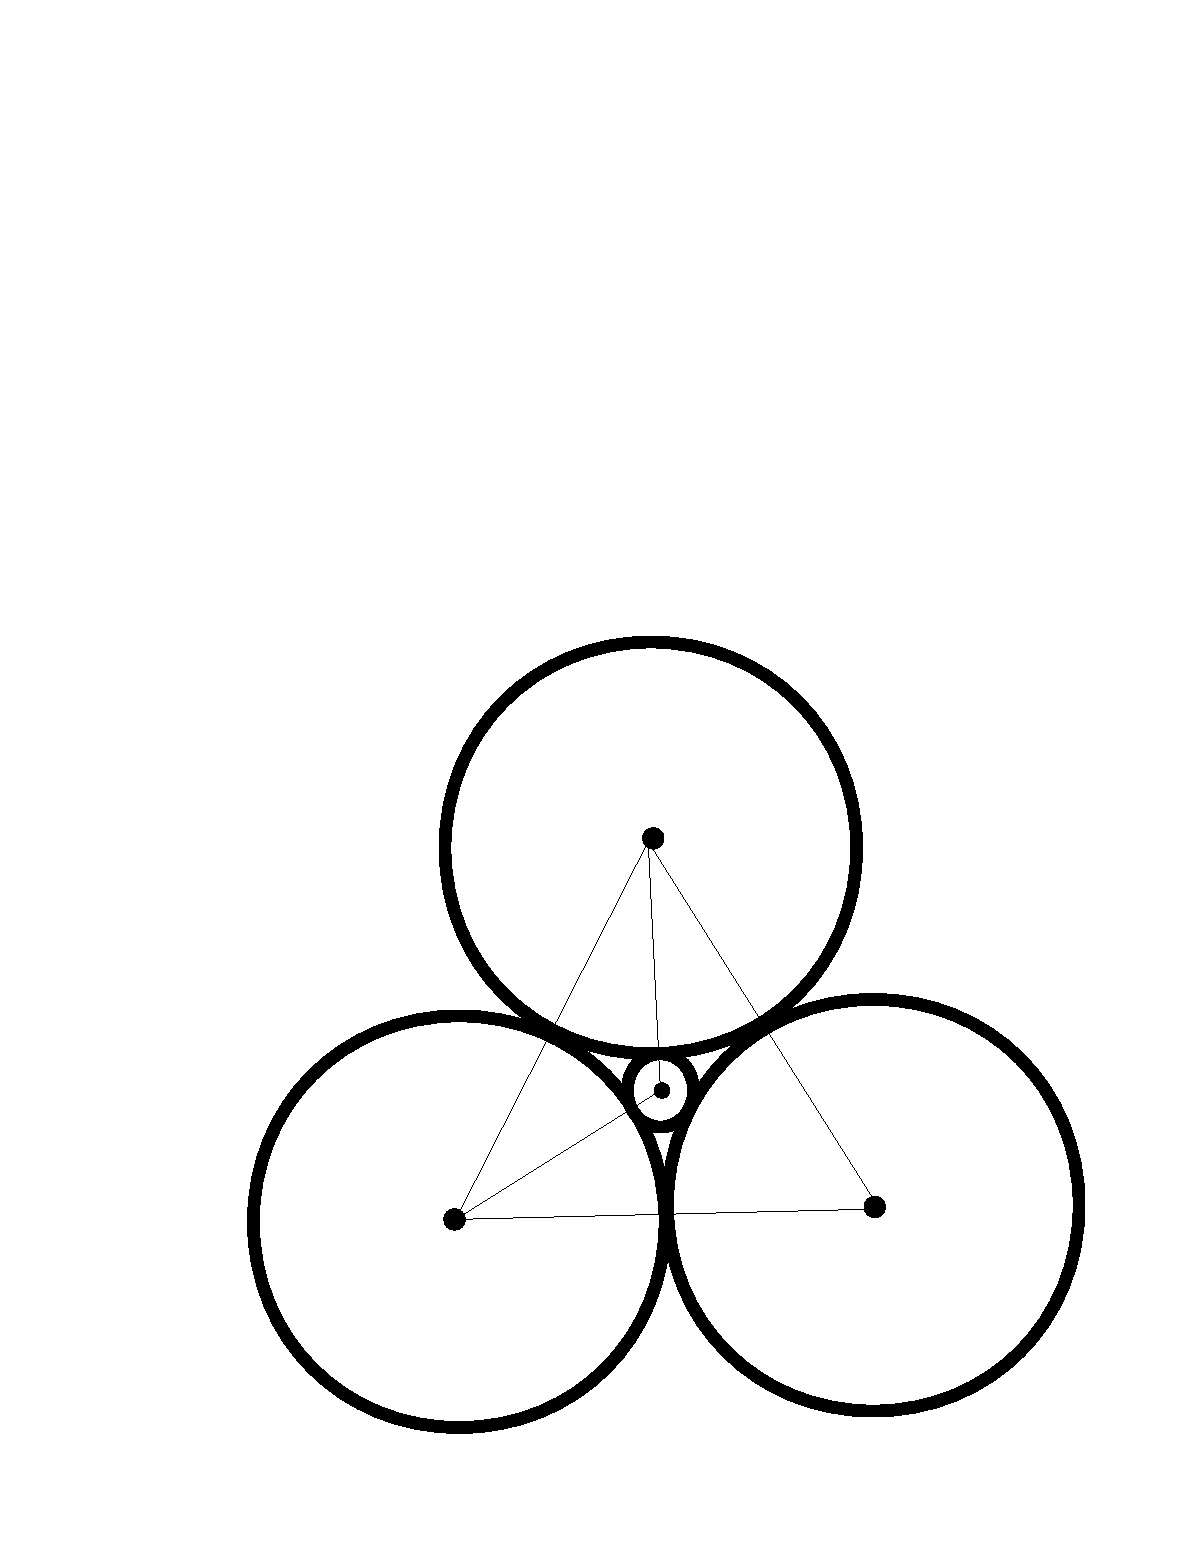
\includegraphics[width=30mm,viewport=106 49 515 440]{CCSPR74-18pic2.eps}
\end{wrapfigure}

\textbf{The correct answer is (A): $\frac{2\sqrt{3}-3}{3}$}\\[1 ex]
Let $r$ be the radius of the small circle. If an equilateral triangle is drawn connecting the centres of the large circles, and lines are drawn from the centres of two of the large circles to the center of the small circle, symmetry tells us that the angle between these two lines is $120^{\circ}$. The triangle containing this $120^{\circ}$ angle will have two sides of length $1+r$, and one side of length 2. Then, by the Law of Cosines,
\begin{align*}
2^2&=(1+r)^2+(1+r)^2-2(1+r)(1+r)\cos{120}\\
4&=2(1+r)^2-2(1+r)^2\times(-\frac{1}{2})=3(1+r)^2\\
1+r&=\sqrt{\frac{4}{3}}\\
r&=\frac{2}{\sqrt{3}}-1=\frac{2\sqrt{3}-3}{3}.
\end{align*}
%End
\\[5 ex]
%Begin
%Language English
%Source Cariboo College High School Mathematics competition
%Title Junior Preliminary Round 1973
%Question 19
%Subject algebra
%Category modelling
%Type MC
%Choices 5
%Answer A
%Creator Victor Semenoff
%Rdifficulty 26
%Qtext

\scriptsize
Source: Cariboo College High School Mathematics Contest

\normalsize
\begin{wrapfigure}[4]{r}[0pt]{0pt}
	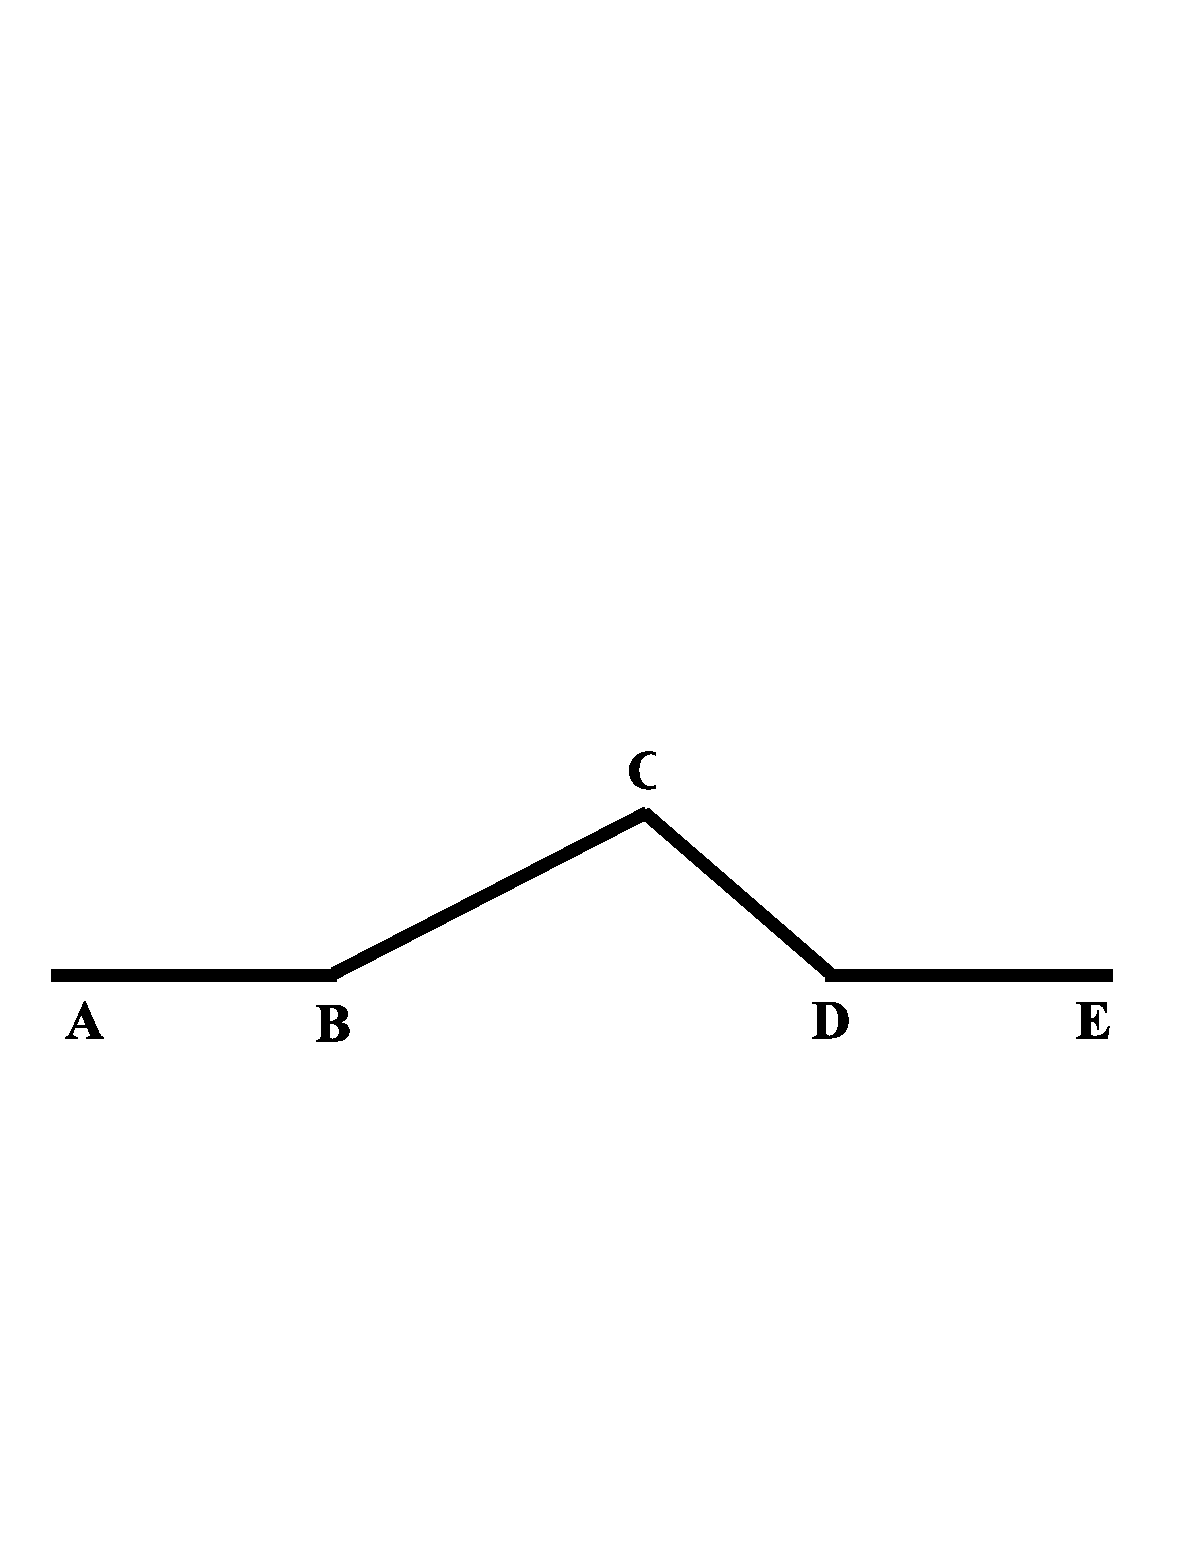
\includegraphics[width=30mm,viewport=11 234 533 389]{CCSPR74-19pic.eps}
\end{wrapfigure}
Antonio makes a journey from A to E and back again on his bicycle. On the level stretches, AB and DE, his average speed is 20km/h. Up the long hill, BC, he averages 12km/h, and down the same hill he averages 24km/h. Down the steeper hill CD, he averages 30km/h, and up this hill he averages 10km/h. If AB=CD=DE, and BC=2AB, then the ratio of Antonio's time to go from A to E to the time for the return journey (E to A) is:\\
%ChoiceA
(A) 18:17\\[1 ex]
%ChoiceB
(B) 37:41\\[1 ex]
%ChoiceC
(C) 59:47\\[1 ex]
%ChoiceD
(D) 41:37\\[1 ex]
%ChoiceE
(E) 12:11\\
%Ftext

\begin{wrapfigure}{r}[0pt]{0pt}
	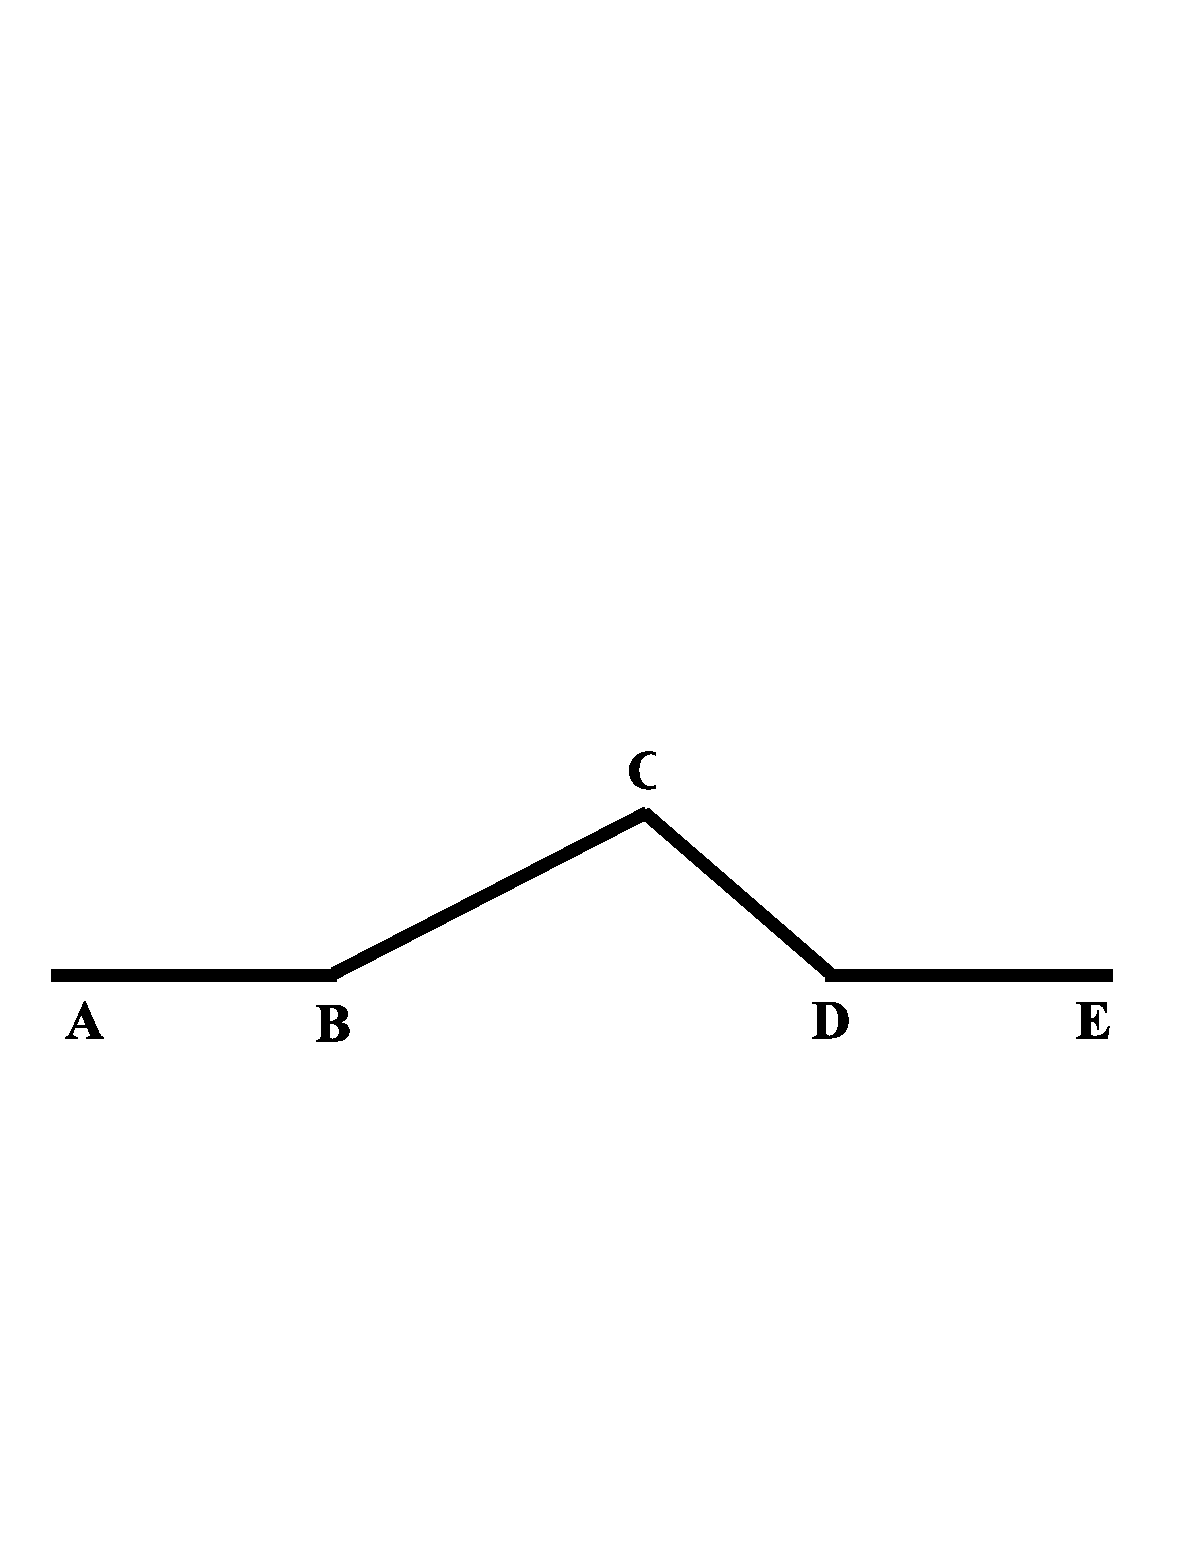
\includegraphics[width=30mm,viewport=11 234 533 389]{CCSPR74-19pic.eps}
\end{wrapfigure}

\textbf{The correct answer is (A): 18:17}\\[1 ex]
Let $t_{mn}$ be the time it takes to travel from point $m$ to point $n$. Similarly let $v_{mn}$ be his speed between these points, and let $d_{mn}$ be the distance. The total time for the one way trip is:
\begin{align*}
t_{\textrm{AE}}&=t_{\textrm{AB}}+t_{\textrm{BC}}+t_{\textrm{CD}}+t_{\textrm{DE}}=\frac{d_{\textrm{AB}}}{v_{\textrm{AB}}}+\frac{d_{\textrm{BC}}}{v_{\textrm{BC}}}+\frac{d_{\textrm{CD}}}{v_{\textrm{CD}}}+\frac{d_{\textrm{DE}}}{v_{\textrm{DE}}}\\
&=\frac{d_{\textrm{AB}}}{20}+\frac{d_{\textrm{BC}}}{12}+\frac{d_{\textrm{CD}}}{30}+\frac{d_{\textrm{DE}}}{20}=\frac{18}{60}d_{\textrm{AB}},
\end{align*}
While the time for the return trip is
\begin{align*}
t_{\textrm{EA}}&=t_{\textrm{ED}}+t_{\textrm{DC}}+t_{\textrm{CB}}+t_{\textrm{BA}}=\frac{d_{\textrm{ED}}}{v_{\textrm{ED}}}+\frac{d_{\textrm{DC}}}{v_{\textrm{DC}}}+\frac{d_{\textrm{CB}}}{v_{\textrm{CB}}}+\frac{d_{\textrm{BA}}}{v_{\textrm{BA}}}\\
&=\frac{d_{\textrm{ED}}}{20}+\frac{d_{\textrm{DC}}}{10}+\frac{d_{\textrm{CB}}}{24}+\frac{d_{\textrm{BA}}}{20}=\frac{17}{60}d_{\textrm{AB}}.
\end{align*}
Therefore, the ratio of Antonio's time to go from A to E to the time for the return journey is
\begin{equation*}
t_{\textrm{AE}}:t_{\textrm{EA}}=18:17.
\end{equation*}
%End
\\[5 ex]
%Begin
%Language English
%Source Cariboo College High School Mathematics competition
%Title Junior Preliminary Round 1973
%Question 20
%Subject geometry
%Category length
%Type MC
%Choices 5
%Answer B
%Creator Victor Semenoff
%Rdifficulty 29
%Qtext

\scriptsize
Source: Cariboo College High School Mathematics Contest

\normalsize
\begin{wrapfigure}[6]{r}[0pt]{0pt}
	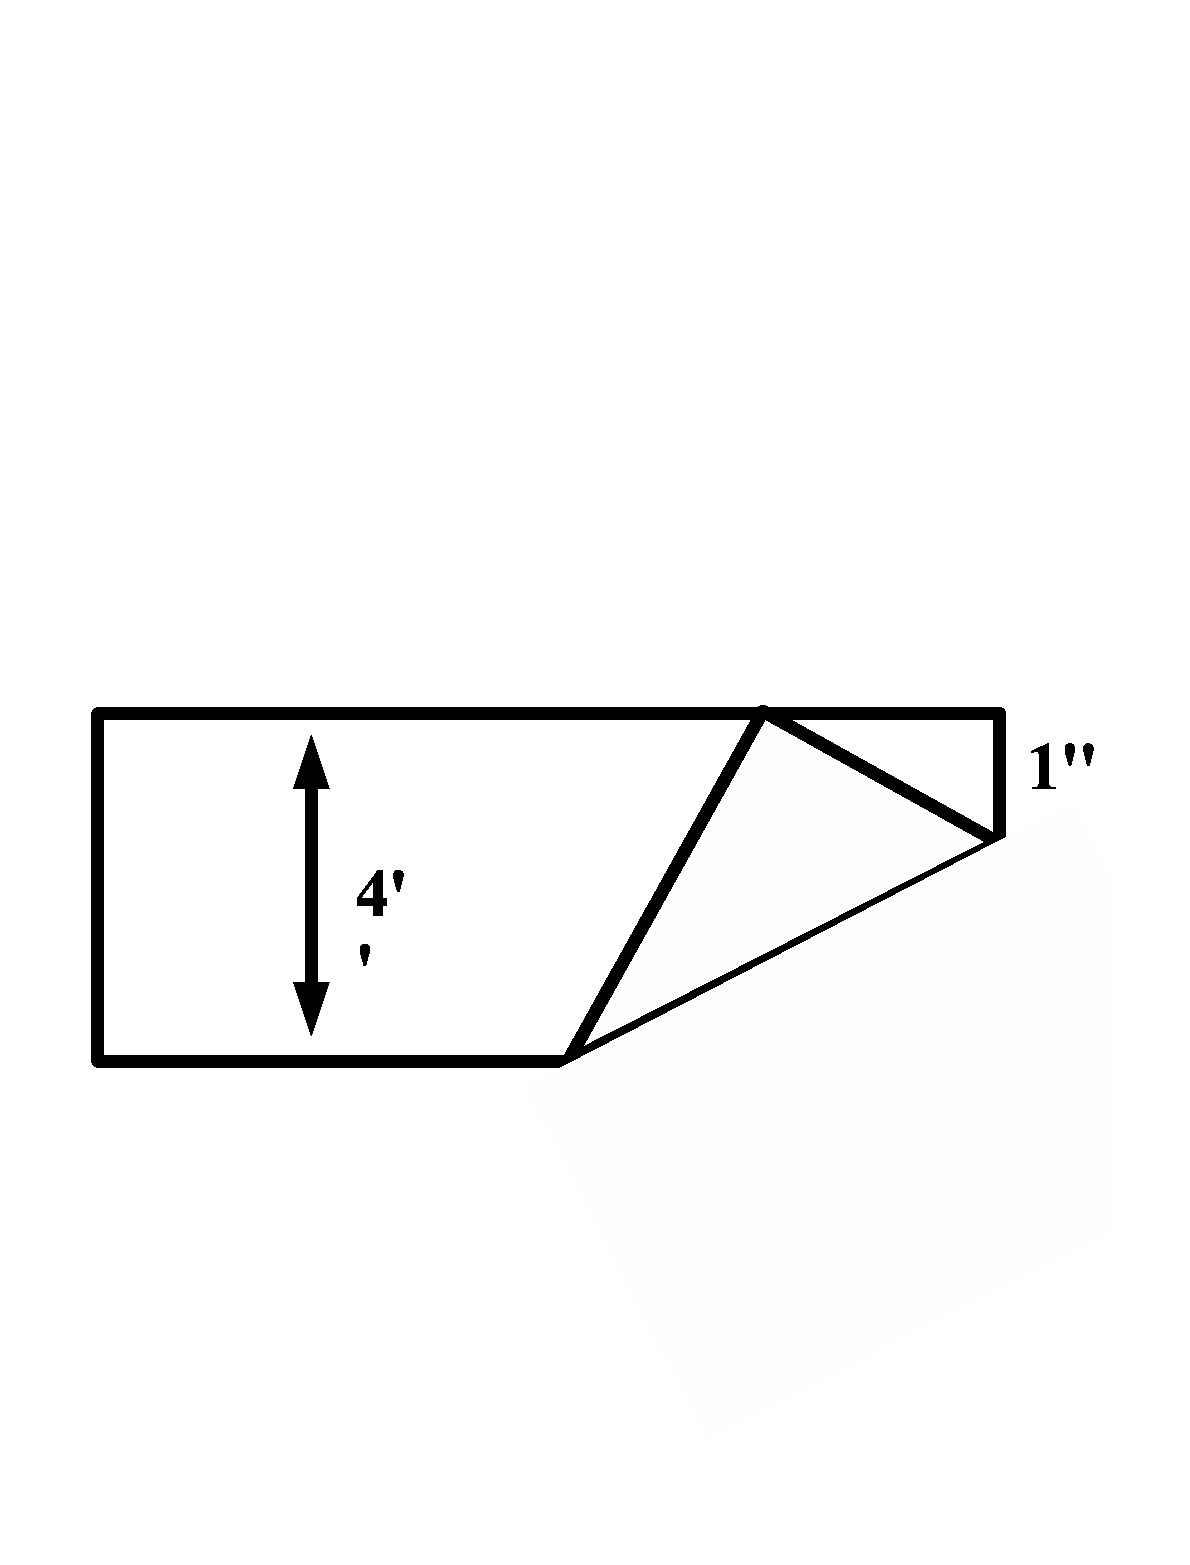
\includegraphics[width=30mm,viewport=29 220 524 411]{CCSPR74-20pic.eps}
\end{wrapfigure}
A rectangular strip of paper 4 inches wide is folded from a point 1 inch below the top right corner, so that the bottom right-hand corner just reaches the top side of the strip. What is the length of the fold (in inches)?\\
%ChoiceA
(A) $3\sqrt{2}$\\
%ChoiceB
(B) $3\sqrt{3}$\\
%ChoiceC
(C) $\frac{3\sqrt{6}}{2}$\\
%ChoiceD
(D) $2\sqrt{2}$\\
%ChoiceE
(E) 5\\
%Ftext

\begin{wrapfigure}{r}[0pt]{0pt}
	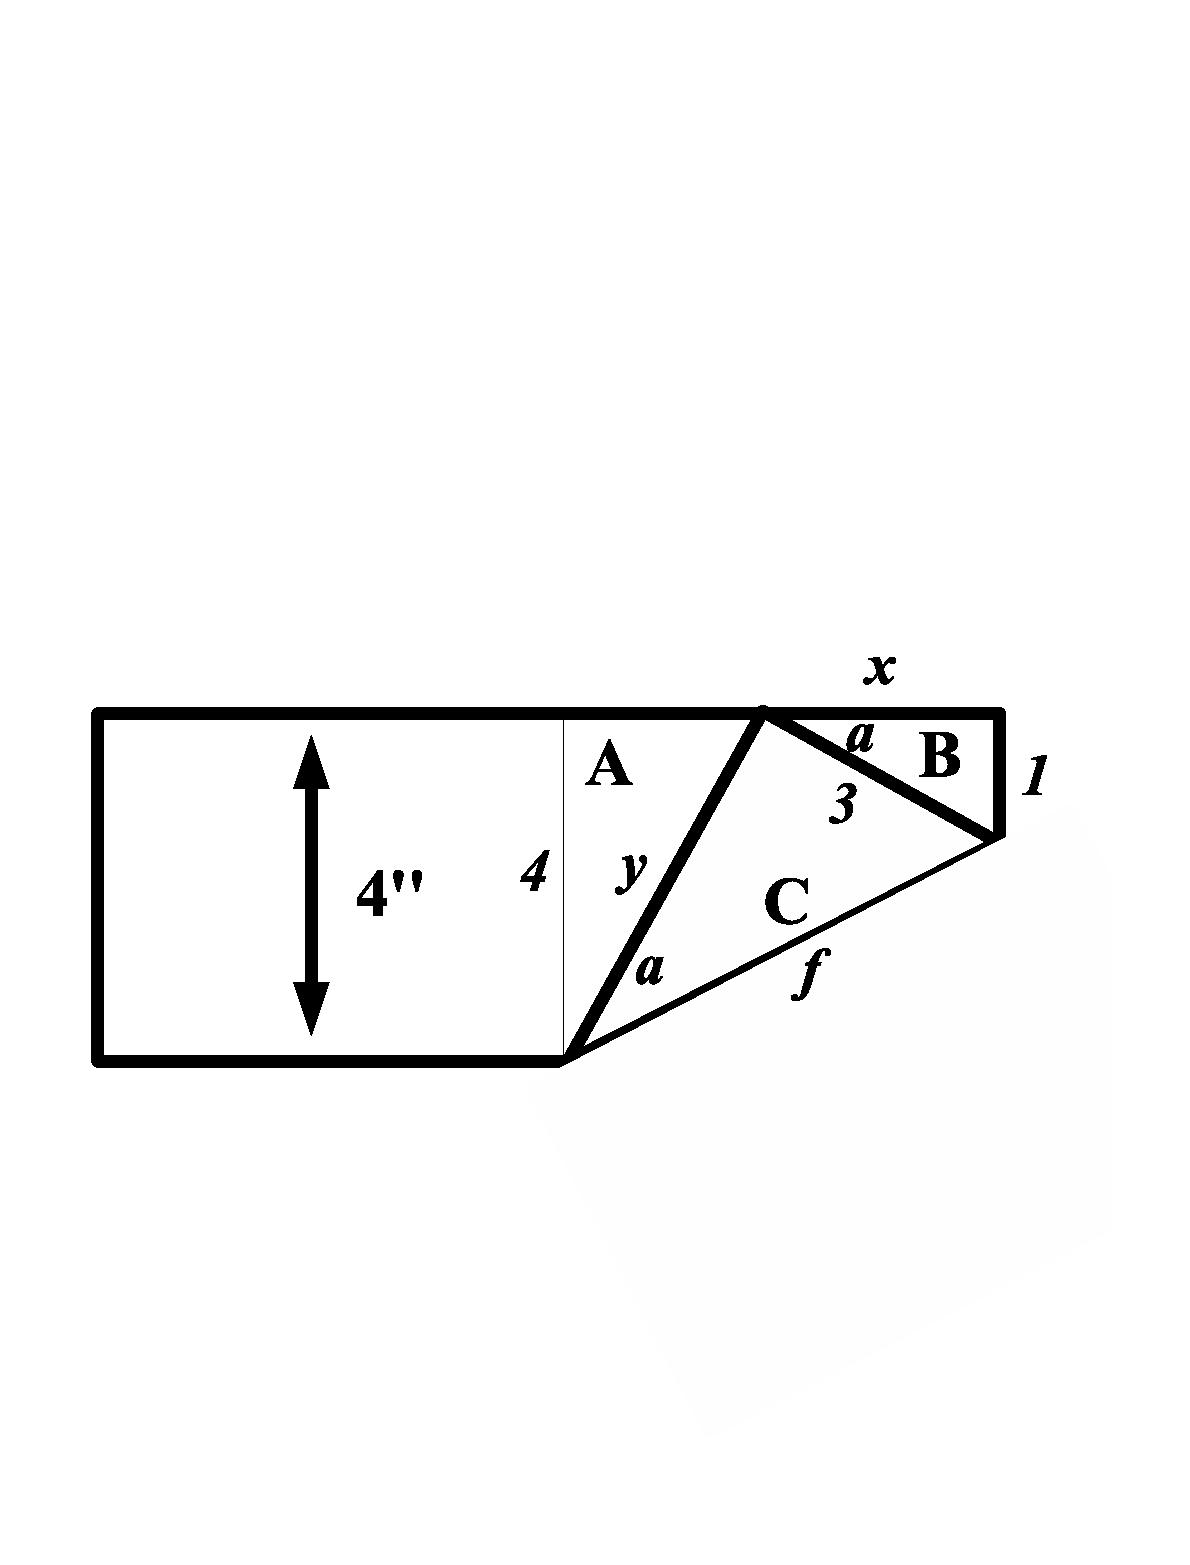
\includegraphics[width=30mm,viewport=29 220 500 431]{CCSPR74-20pic2.eps}
\end{wrapfigure}

\textbf{The correct answer is (B): $3\sqrt{3}$}\\[1 ex]
Since the horse can run $1\frac{1}{4}=\frac{5}{4}$ miles in the same time the man can run $\frac{1}{2}$ mile, the ratio of their speeds is
\begin{equation*}
\frac{5}{4}:\frac{1}{2}=5:2.
\end{equation*}
From Pythagoras, we have $1^2+x^2=3^2$, thus $x=\sqrt{8}$. Also, triangles A and B are similar, thus
\begin{equation*}
\frac{y}{4}=\frac{3}{x}.
\end{equation*}
Substituting in $x=\sqrt{8}$, we get $y=\frac{6}{\sqrt{2}}$. By the Pythagoras Theorem on triangle C, we find
\begin{align*}
3^2+y^2&=f^2\\
f^2&=9+18\\
f&=\sqrt{27}=3\sqrt{3}
\end{align*}
Thus the length of the fold is $3\sqrt{3}$ inches.
%End
\end{document}
